%==============================================================================
\section{Simulation Input}
\label{sec:sim_input}
%==============================================================================

In this section, the actual values of the inputs required by \papa as described
in Sec.~\ref{sec:papa_code} will be presented as they were used to generate the
results reported in Sec.~\ref{sec:results_baseline}. The detector-related
inputs were extracted from the official PINGU Monte Carlo datasets for geometry
V36\footnote{These are the PINGU Monte Carlo runs 390 for \nue and \nuebar, 389
for \numu and \numubar, and 390 for \nutau and \nutaubar.}.

\subsection{Atmospheric Neutrino Flux}
\label{sec:input_flux}

\begin{figure}[htbp]
 \centering
 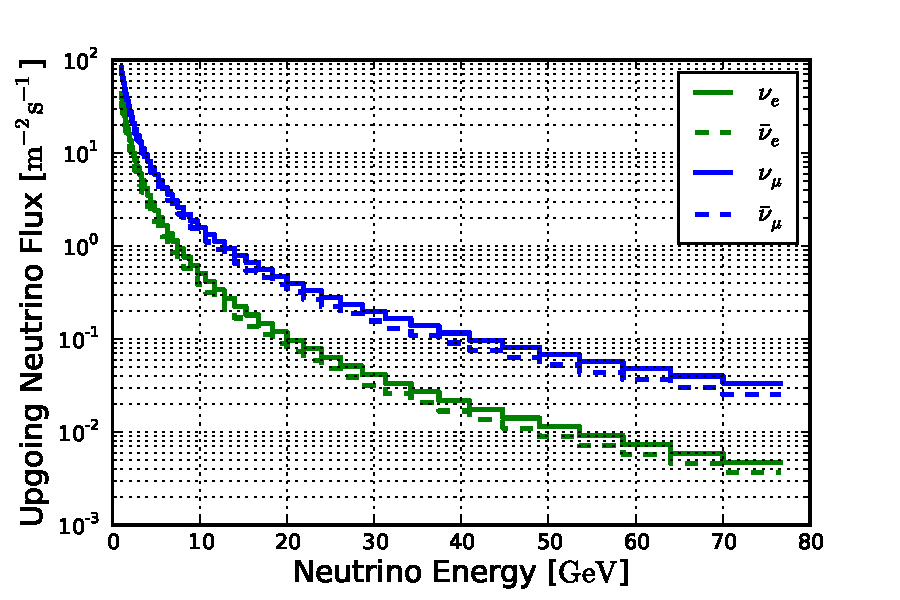
\includegraphics[width=0.7\linewidth]{summed_flux}
 \caption{The atmospheric neutrino flux at the South Pole integrated over all
          upgoing (\coszen in $[-1,0]$) directions. Based on the
          azimuth-averaged neutrino flux tables from \cite{HondaSP}.}
\label{fig:summed_flux}
\end{figure}

As already mentioned, the incoming atmospheric neutrino flux without
oscillations is calculated from the 2014 re-calculation of the flux tables
published by Honda et al.\ \cite{Honda, HondaSP}. A plot of the flux in the
energy range covered by the PINGU simulation (1\,--\,80\,GeV) is shown in
Fig.~\ref{fig:summed_flux}. The flux has been integrated over all upgoing
(\coszen in $[-1,0]$) directions, as downgoing neutrinos arriving from above
the detector do not pass through a significant amount of matter and hence do
not bear any information on the neutrino mass hierarchy.

\subsection{Oscillation Probabilities}
\label{sec:input_osc}

The neutrino oscillation probabilities have been calculated using the
AtmoWeights code for the PREM Earth density profile as described in
Sec.~\ref{sec:PINGUosc}. The fiducial values of the mixing parameters used for
the calculation follow the global fit of Fogli et al.\ \cite{Fogli}, listed in
Tab.~\ref{tab:fiducial_osc}. Example plots of the probabilities demonstrating
the characteristic signature of the mass hierarchy are shown in high resolution
in that section as well, the full set of all possible oscillation channels can
be found in App.~\ref{app:oscillation}. The binning of those plots is the same
as used for the actual analysis, which is 79 logarithmic bins in energy between
1\,GeV and 80\,GeV and 20 equally sized bins between -1 and 0 in \coszen.

\subsection{Effective Areas}
\label{sec:input_aeff}

\begin{figure}[htbp]
 \centering
 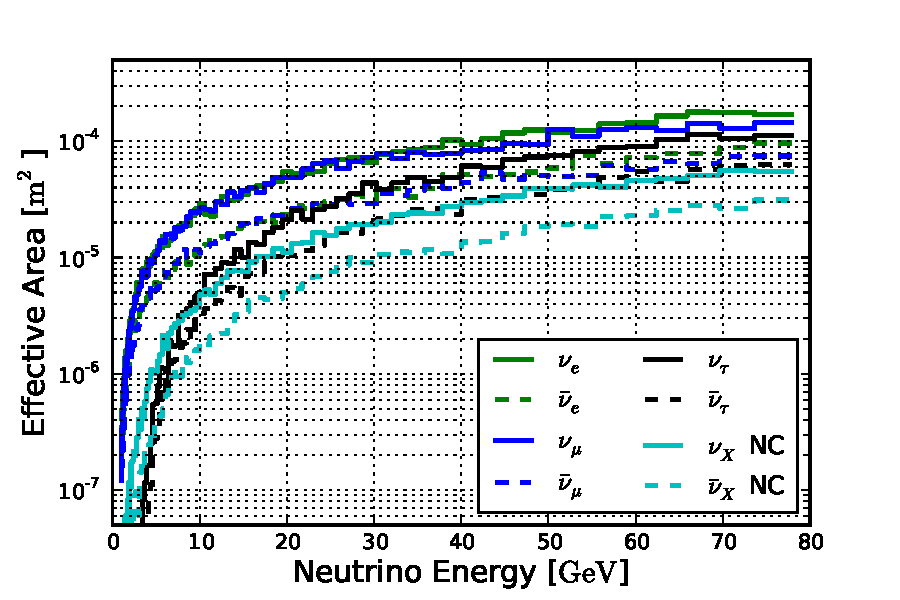
\includegraphics[width=0.495\linewidth]{aeff_energy}
 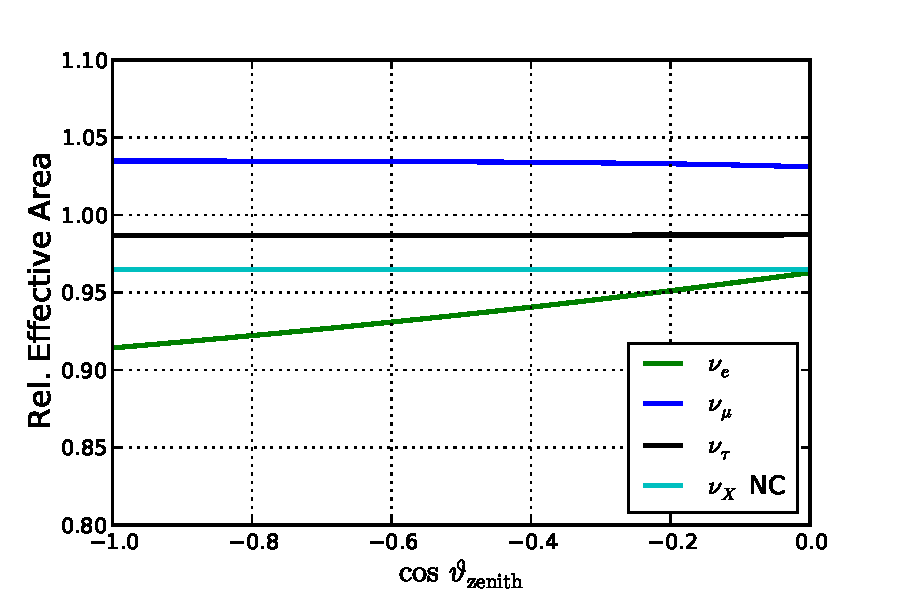
\includegraphics[width=0.495\linewidth]{aeff_coszen}
 \caption{Effective areas for all relevant neutrino interactions. Shown are
  energy (left)  and zenith (right) dependence.}
\label{fig:aeffs}
\end{figure}

The effective areas are extracted from PINGU Monte Carlo datasets via the
OneWeight quantity multiplied by $4\pi$, which is equivalent to a per-event
effective area \cite{OneWeight}. The zenith dependence of the effective area is
modelled by an analytic fit to the MC data, assuming that energy and zenith
dependence can be handled separately. A plot of the effective areas and their
zenith dependence is shown in Fig.~\ref{fig:aeffs}.

\subsection{Reconstruction Resolutions}
\label{sec:input_reco}

\begin{figure}[p]
 \centering
 $\begin{array}{cc}
   \mathrm{Energy\ Resolution} &
   \mathrm{\coszen\ Resolution}\\
   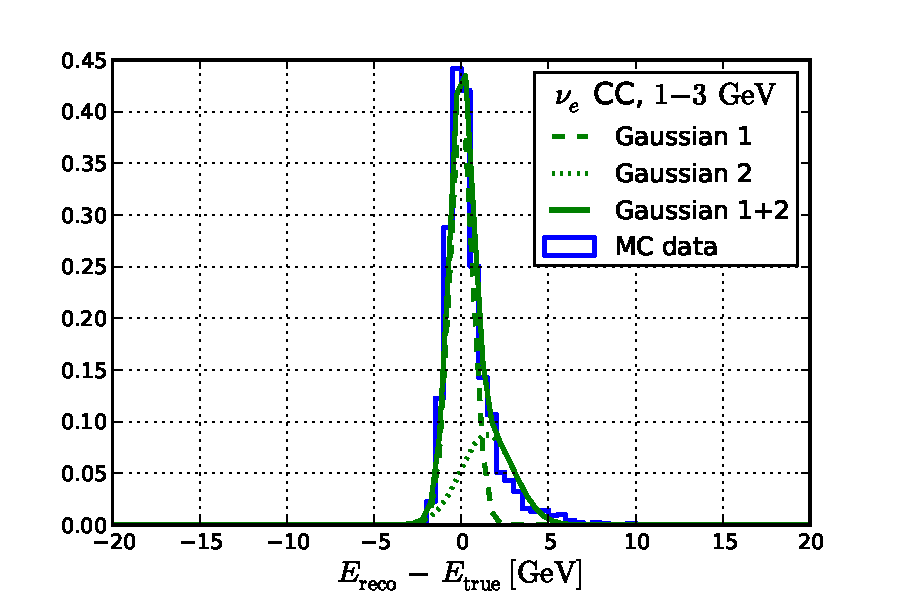
\includegraphics[width=0.5\columnwidth]{e_reco_nue_2GeV} &
   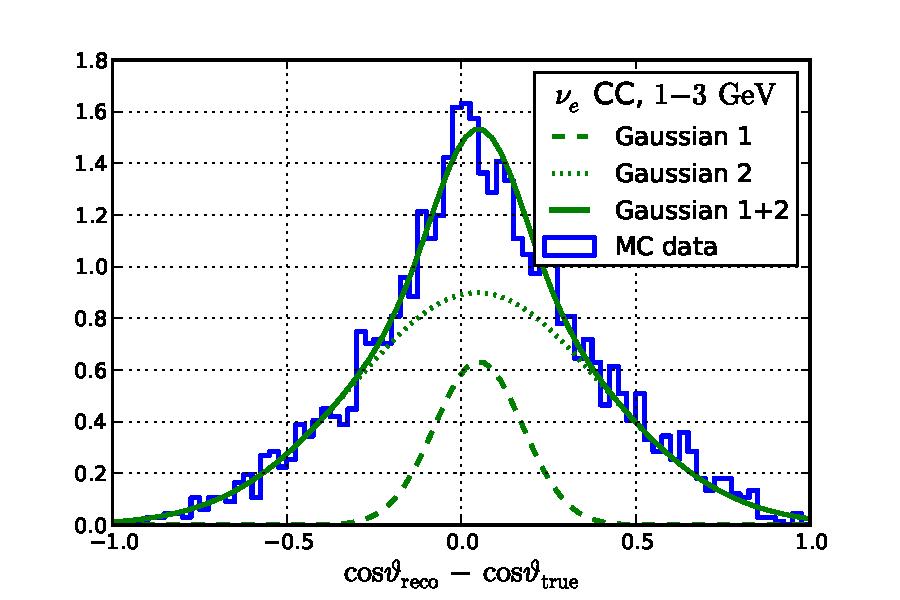
\includegraphics[width=0.5\columnwidth]{cz_reco_nue_2GeV}\\
   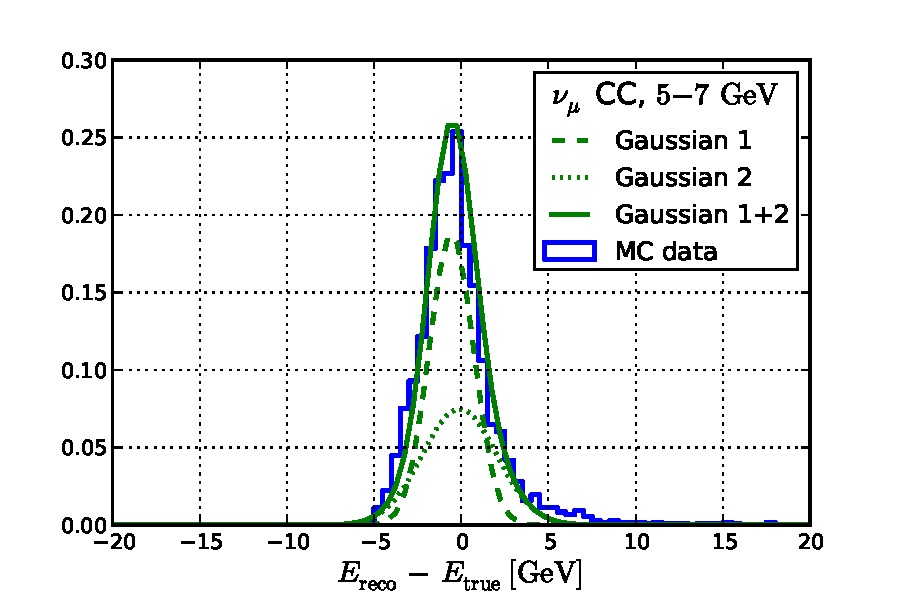
\includegraphics[width=0.5\columnwidth]{e_reco_numu_6GeV} &
   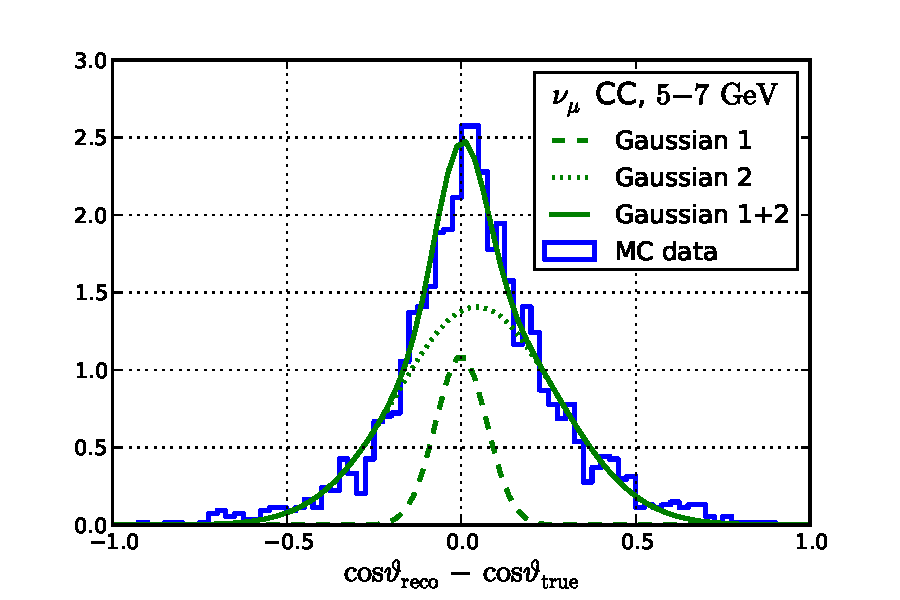
\includegraphics[width=0.5\columnwidth]{cz_reco_numu_6GeV}\\
   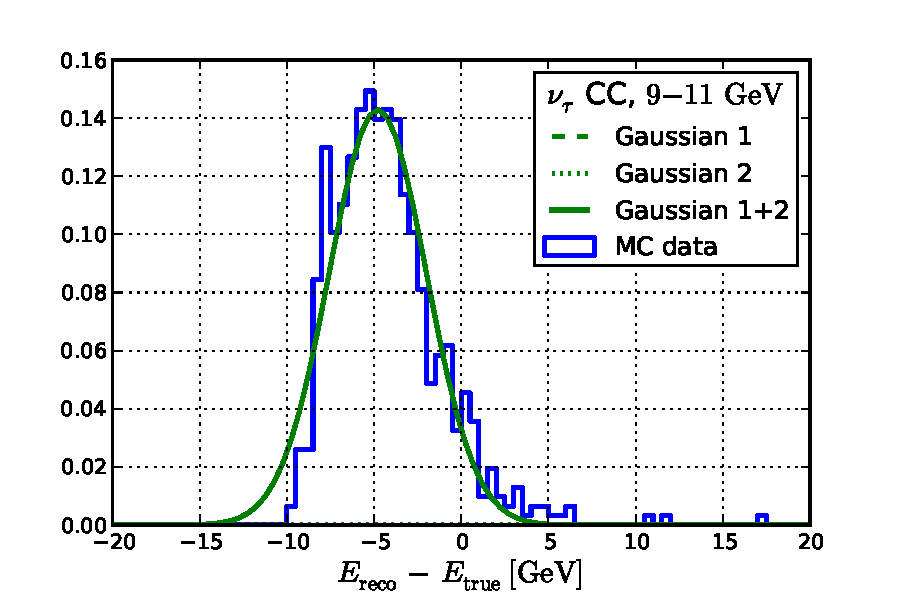
\includegraphics[width=0.5\columnwidth]{e_reco_nutau_10GeV} &
   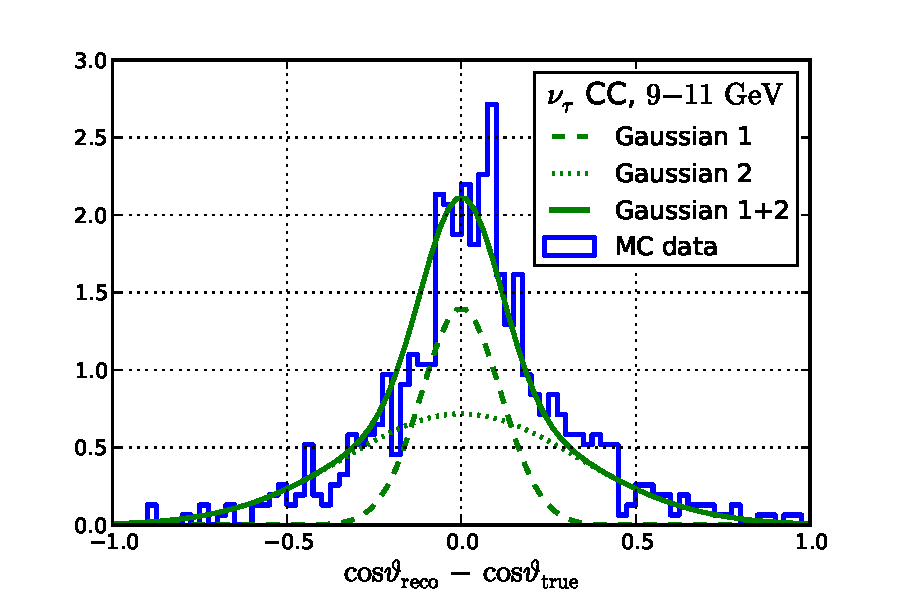
\includegraphics[width=0.5\columnwidth]{cz_reco_nutau_10GeV}\\
   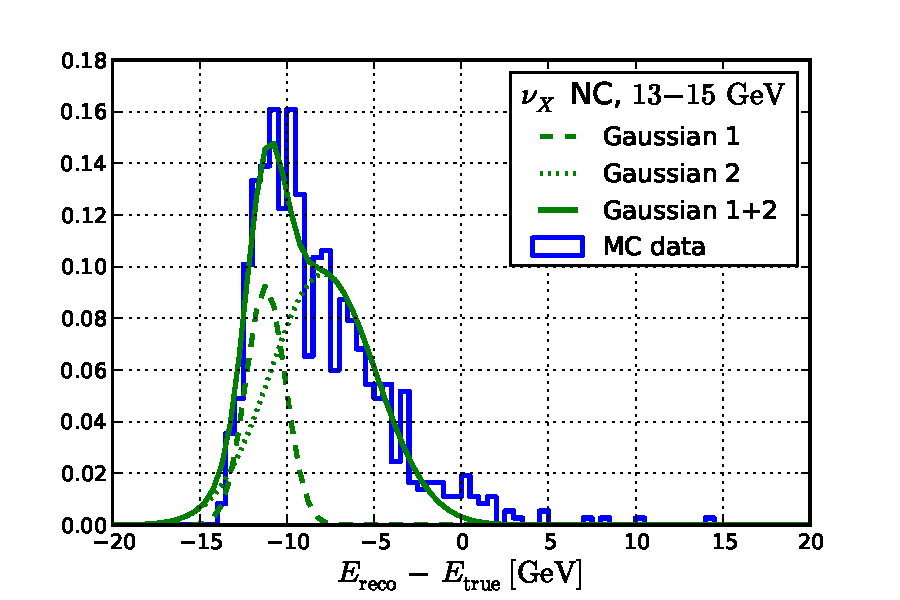
\includegraphics[width=0.5\columnwidth]{e_reco_NC_14GeV} &
   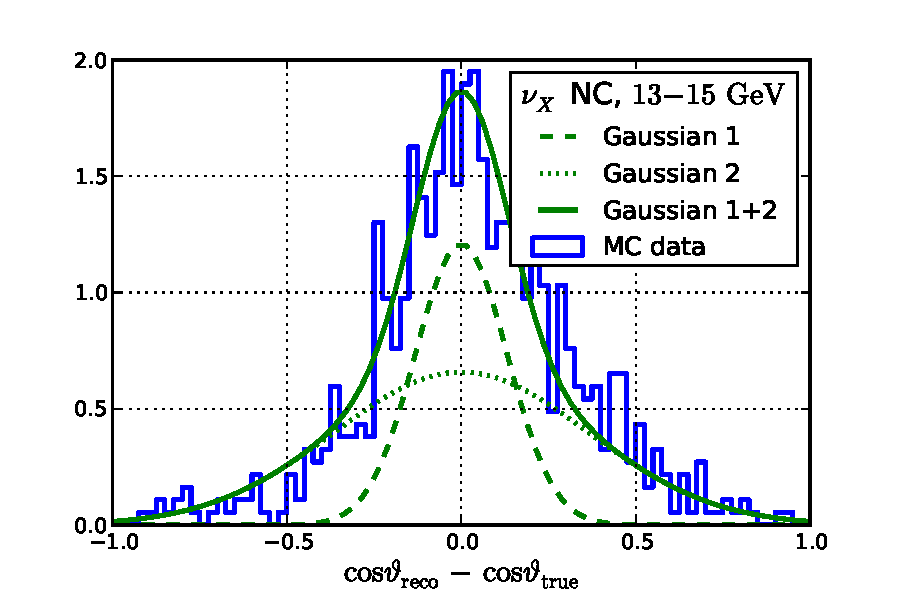
\includegraphics[width=0.5\columnwidth]{cz_reco_NC_14GeV}
  \end{array}$
 \caption{Examples for the parametrisations of the energy (left) and \coszen
   (right) reconstruction resolutions for (from top to bottom) \nue, \numu, and
   \nutau CC and \nux NC events.
   Note the bias towards low reconstructed energies for \nutau and NC.
   }
 \label{fig:reco_example}
\end{figure}

The event reconstruction for the baseline model will be simulated by smearing
the 2D event histograms with kernels represented by the sum of two Gaussian
distributions (cf.~Sec.~\ref{sec:papa_code}). The five parameters needed to
describe these Gaussians, see (\ref{eqn:reco_param}), are given as functions of
the neutrino energy. To get the energy dependence of these five parameters, a
two-stage fitting procedure is applied. 

In the first stage, all events of a given interaction channel are divided into
subsets according to their true neutrino energy, where each subset covers an
energy range of 2\,GeV. For each of the subsets up to an energy of
20\,GeV\footnote{At higher energies, the event statistics are too low for the
fit to converge.}, the difference between true and reconstructed energy is
histogrammed and fitted with the aforementioned kernel function. This results in
values for the five parameters of (\ref{eqn:reco_param}) as a function of
energy. These are fitted again, now as (piecewise) linear functions of the true
neutrino energy.

After repeating the procedure for the resolution in \coszen, the fit function
definitions are stored in a dictionary that serves as input to \papa. This
dictionary can be found in App.~\ref{app:reco_params}. For the actual fits to
the resolutions, examples are shown in Fig.~\ref{fig:reco_example}. In the
\nutau CC and \nux NC interaction channels, the reconstructed energies are
biased towards too low values. This is a result of the neutrinos in the
respective final states which is not detected and hence carries away
``missing energy'' (cf.~Sec.~\ref{sec:XsecsGeV}).

Although the fits are only anchored to data up to 20\,GeV, they are extrapolated
to higher energies. This approach is valid as events beyond 20\,GeV are so far
above PINGU's energy threshold that new features in the description of the
reconstruction resolutions are not to be expected. In addition, the mass
hierarchy signature is located at energies below 10\,GeV (see
Figs.~\ref{fig:true_akhmedov_nue} -- \ref{fig:true_akhmedov_nutau}), such that
inaccuracies in the resolution parametrisations above 20\,GeV do not influence
the calculation of the mass hierarchy sensitivity.

\subsection{Particle Flavour Identification}
\label{sec:input_pid}

\begin{figure}[htbp]
 \centering
 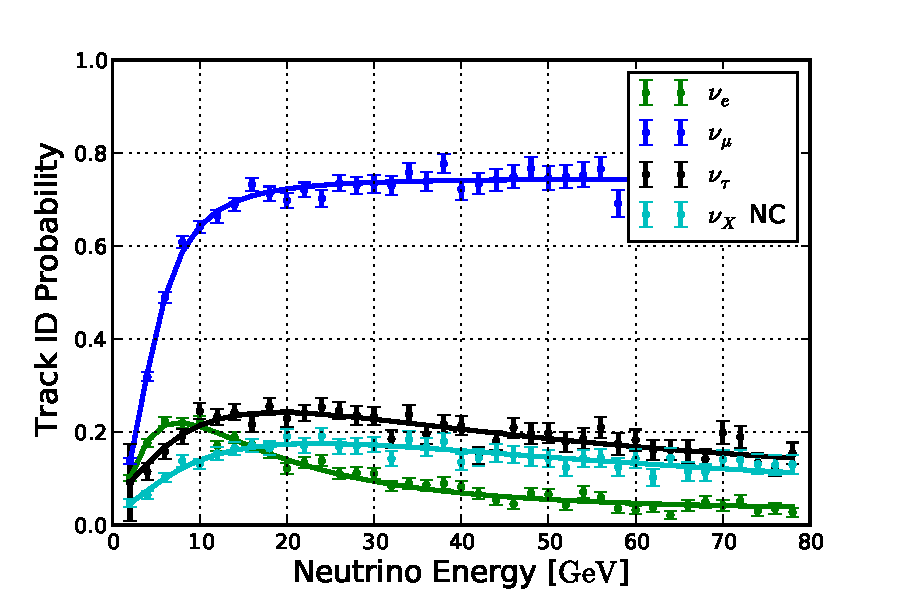
\includegraphics[width=0.7\textwidth]{PID}
 \caption{Track identification probability as function of energy in all four
  interaction channels. The straight lines show fits to the data.}
 \label{fig:PID}
\end{figure}

The classification of the neutrino events into track-like and cascade-like
events is according to their final score in the boosted decision tree described
in Sec.~\ref{sec:cuts_PID}. In the baseline detector settings, the decision is
of binary nature, meaning that the probability to classify a given event as
cascade is one minus the probability to classify it as a track.

Data points for the track identification probabilities in all channels as a
function of the neutrino energy have been provided by \cite{JP_PID}. These data
were fitted with analytic functions, the fits are shown together with the data
points in Fig.~\ref{fig:PID}. The functions definitions themselves are listed
in App.~\ref{app:pid}.